\documentclass{article}
\usepackage{amsmath}
\usepackage{amssymb}
\usepackage{graphicx}
\usepackage{subcaption}
\usepackage[utf8]{inputenc}
\usepackage[table]{xcolor}
\usepackage[margin=1.2in]{geometry}


\usepackage{lipsum}

\title{Statistical Mean Reversion of \\
Airline and Oil Company Stock Prices \\
\large CSC 265 Final Project}
\author{Dominick Harasimiuk - 30702462\\
Source Code Available At:\\ 
https://github.com/DominickH20/statistical-mean-reversion}
\date{May 7, 2021}


\begin{document}
\maketitle

\vspace{1cm}

\begin{abstract}
\noindent
\lipsum[1]
\end{abstract}

\newpage
\section{Introduction}
The intent of this project is to build a reliable statistical mean reversion trading strategy
on correlated baskets of stocks, specifically airline and oil company stocks. Airline companies
are exposed to very similar pools of risk, and the same can be said for oil companies. Because
of this, one would expect their stock prices to move together when these underlying risk
factors change. Because airlines are large consumers of oil, one might expect the airline and
oil sectors to exhibit some relationship as well.
\subsection{Statistical Mean Reversion}
This project aims to develop a model for how these companies behave in relation
to one another. This model can be thought of as the "mean" in this mean reversion concept. I
utilize this model in the context of a trading strategy by computing the expected stock return 
at time $t$, call it $e_t$. The expected return can be compared to the actual return, $a_t$
at that same time period $t$. This generates a residual, $r_t = a_t - e_t$. If this residual
is sufficiently positive, then the strategy concludes that the stock in question has grown too 
much over the period, so it would sell. Likewise, if the $r_t$ is sufficiently negative, then the 
strategy judges that stock has underperformed over the period relative to its peers, so it would buy. In both cases
the strategy is betting on convergence to the statistical relationship between the securities.
In this paper, I outline such strategies on pairs of securities as well as baskets of securities,
using principal component analysis to handle the multicollinearity problem for regression
models implemented on such data.

\subsection{Data}
\subsubsection{Scope}
The data used in the subsequent analyses were obtained from the Alpaca Markets historical 
market data API. The securities examined in this study are the following: American Airlines
(AAL), Delta Airlines (DAL), Southwest Airlines (LUV), Allegiant Airlines (ALGT), United
Airlines (UAL), Chevron (CVX), Marathon Oil (MRO), Murphy Oil (MUR), Exxon Mobil (XOM),
Devon Energy (DVN), SPDR S\&P 500 ETF, and iShares Treasury Bond ETF (TLT). There 
are 5 airline companies, 5 oil companies, and 2 market factors (SPY and TLT). The motivation
behind including the market factors in this study is that they help parameterize what is going
on in equity and debt markets at any given point in time.
\subsubsection{Data Format}
The data range from
the start of 2016 to May 1st 2021. The years 2020 and 2021 are held out as test data while the
rest of the data is used to train the models. Given the occurrence of the pandemic in 2020,
this is a particularly challenging test set. The data is organized in a \textit{bar} format.
Bars are a common way of aggregating financial data and are structured as follows:
$$B_{S} = \begin{bmatrix} \mathrm{bar}_0, & \mathrm{bar}_1, & 
    ..., & \mathrm{bar}_n \end{bmatrix}$$
$$\mathrm{bar}_i = \begin{bmatrix} \mathrm{datetime}_i & \mathrm{open}_i & 
    \mathrm{high}_i & \mathrm{low}_i & \mathrm{close}_i & \mathrm{volume}_i 
\end{bmatrix}$$
Where $S$ is some security, and $B_S$ is the bar set for that security. Each bar summarizes
a section of trading activity. The open and close are the first and last trades occurring within
the timeframe of the bar, while the high and low are the highest and lowest trade prices 
observed within the timeframe of the bar. The volume represents the number of shares that
traded within the bar. For this analysis, only the closing prices are used.
\subsubsection{Data Cleaning}
The data set was cleaned and imputed before use in any models. There were missing bars 
for several securities, so the most abundant time series (SPY) was used as a baseline for 
bar availability. For every bar in SPY, if there was not an analagous bar present in each 
other security, $S$, then the most recent bar in $S$ was backfilled in its place. 

There were
also several outliers present in the data that would obstruct the fitting of linear models. 
\begin{figure}[h!]
  \centering
  \begin{subfigure}{.5\textwidth}
    \centering
    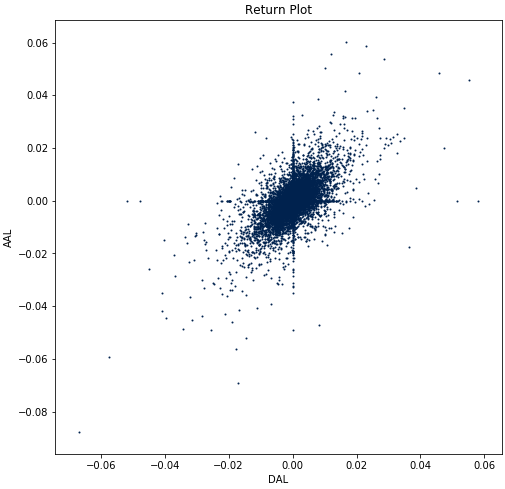
\includegraphics[width=.95\linewidth]{../Figures/return_plot_out.png}
    \caption{Returns with Outliers}
  \end{subfigure}%
  \begin{subfigure}{.5\textwidth}
    \centering
    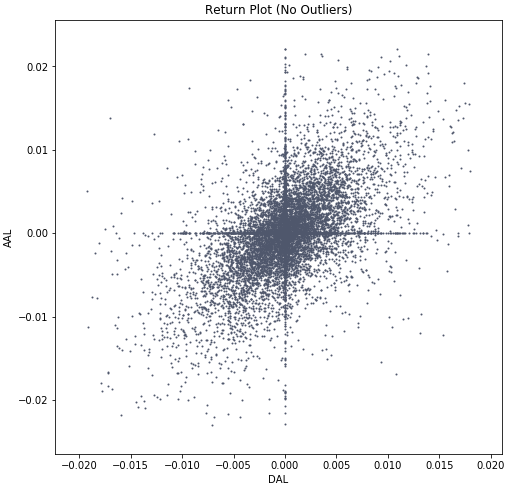
\includegraphics[width=.95\linewidth]{../Figures/return_plot_no_out.png}
    \caption{Returns with Outliers Removed}
  \end{subfigure}
  \caption{Impact of Outliers on Data}
\end{figure}
In order for the models to be able to learn the usual relationship between the securities, I used
the middle 99\% of data \textit{for training only}. The models were still evaluated on train and
test data that included outliers. The outlier removal was solely done to improve the fit of the
linear models.


\subsection{Returns and Markouts}
\subsubsection{Returns}
Asset returns represent 
a scaled first difference in the data, so they eliminate the serial component in the 
time series data along with the complications associated with this. The actual return 
as mentioned above can be defined as follows:
$$a_t = \frac{P_t - P_{t-1}}{P_{t-1}}$$
Normal approximations
have been used for asset returns on the monthly time scale, however, over short intervals this
assumption breaks down. The hourly returns used in this study are abundant close to 0 and 
extreme returns occur with greater frequency than under normality assumptions.
Despite this fact, OLS is a \textit{BLUE} estimator, so we can still confidently estimate 
a line despite the distribution not being normal. 
\subsubsection{Markouts}
Markouts are a way of computing hypothetical trade profits or losses. At every point along the
time series, we hypothetically enter a trade and hold for some predefined number of time 
periods, after which we exit the trade. Note that the entry can be a selling (short selling)
or buying trade, while the exit is simply the opposite side of the entry transaction. To 
specify this more rigorously, we can write:
$$M_{t,k} = \begin{cases} 
P_{t+k} - P_t \text { if Buy}\\
P_t - P_{t+k} \text { if Sell}
\end{cases}$$
This is the markout at time $t$, held for $k$ periods. Notice that $M^B_{t,k} = -M^S_{t,k}$,
meaning that the profit or loss of a buying and selling trade at a given point in time are 
exact opposites (since the asset can only move one direction). A good trading signal is one
that is able to separate positive from negative markouts. 

\section{Pairwise Mean Reversion}
As mentioned in the introduction, airline companies are exposed to similar pools of
risk. Oil companies are also exposed to similar pools of risk. Airline and oil companies
are both exposed to the price risk of oil itself, so it would stand to reason that the
stock prices of companies in this sector would move together. This assumption underpins
the pairwise mean reversion models presented in this section.
\subsection{Pairwise Correlations}
To get an idea of the relationships present among the companies in the data set, a pairwise
correlation analysis was conducted on the hourly returns of each of the securities.
\begin{figure}[h!]
  \centering
    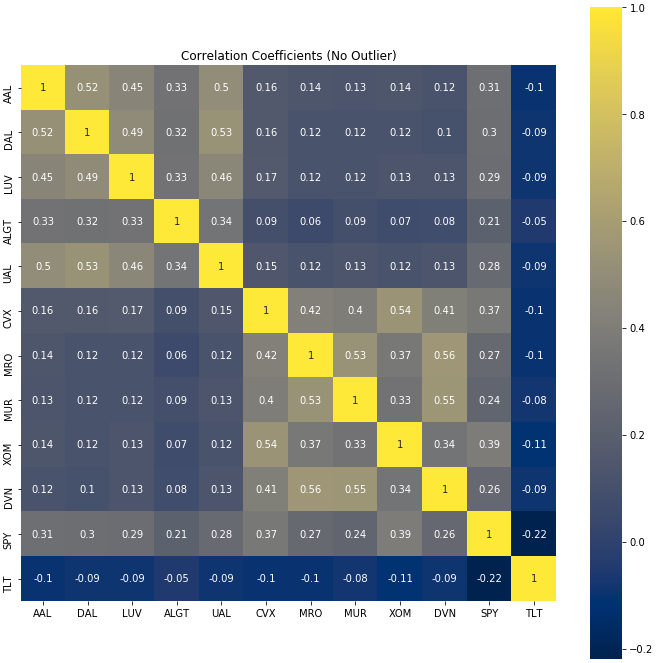
\includegraphics[width=.6\linewidth]{../Figures/pair_corr_no_out.png}
    \caption{Pairwise Correlation - Outliers Removed}
\end{figure}
We can see from Figure 1 above and section 6.3 in the appendix that the outliers in the 
data set had a noticeable positive impact on the correlations between the securities,
so for training purposes, it was appropriate to remove them. There are clear sections
of correlatedness in Figure 2 above. We can see that the 5 airline companies are together
correlated, while the same can be said for the 5 oil companies in the data set. There is also
some positive correlation between the companies in the data set and the S\&P 500 as well as some
negative correlation with price of bonds.

\subsection{Pairwise OLS}
With this understanding of the correlations between the data as well as the fact that
the outlier free return data exhibits ellipsoidal linear relationships, it became clear
that OLS would be a good model for this data. OLS was able to fit lines to the data well,
however, because the data fail to satisfy some assumptions of OLS, inference on the 
OLS parameters was not possible. The coefficients of the pairwise OLS model can be found
in Figure 3(a).
\begin{figure}[h!]
  \centering
  \begin{subfigure}{.5\textwidth}
    \centering
    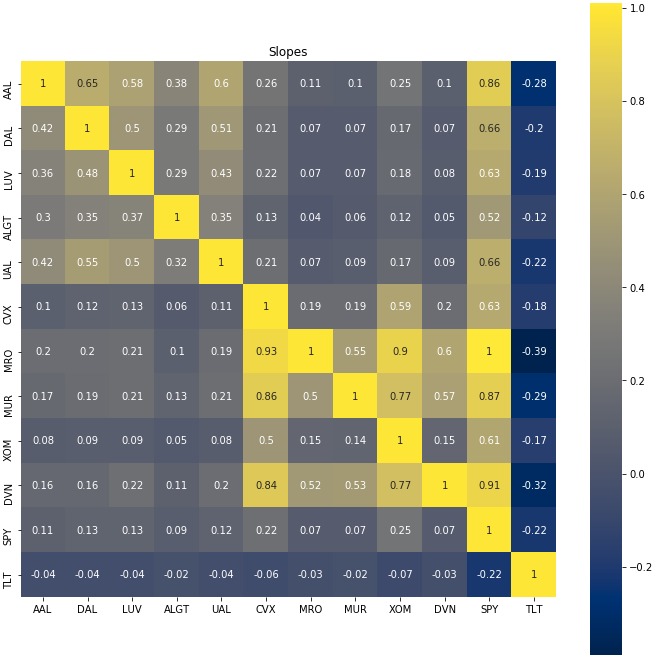
\includegraphics[width=.95\linewidth]{../Figures/pair_reg_slope.png}
    \caption{Model Slope Coefficient}
  \end{subfigure}%
  \begin{subfigure}{.5\textwidth}
    \centering
    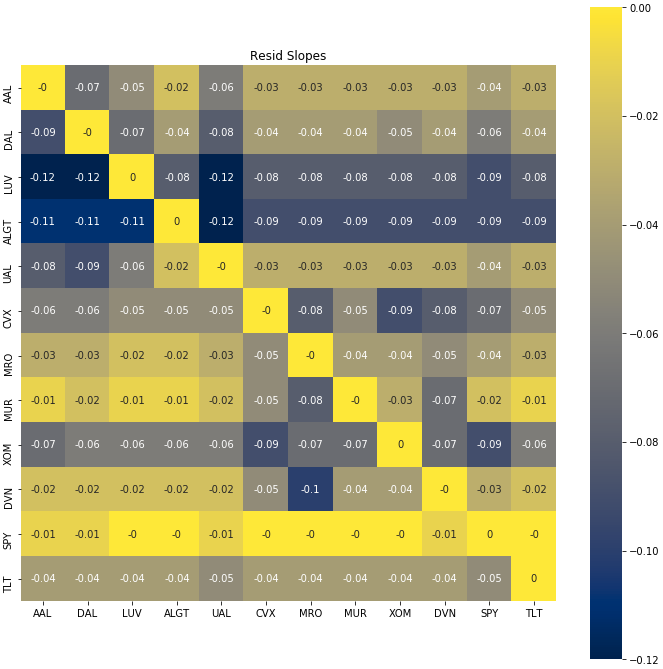
\includegraphics[width=.95\linewidth]{../Figures/pair_resid_reg_slope.png}
    \caption{Residual Slope Coefficient}
  \end{subfigure}
  \caption{Pairwise OLS}
\end{figure}
We see that the the strength of the slope coefficients lines up well with the strength of the
pairwise correlation between the assets. 

\begin{figure}[h!]
  \centering
  \begin{subfigure}{.5\textwidth}
    \centering
    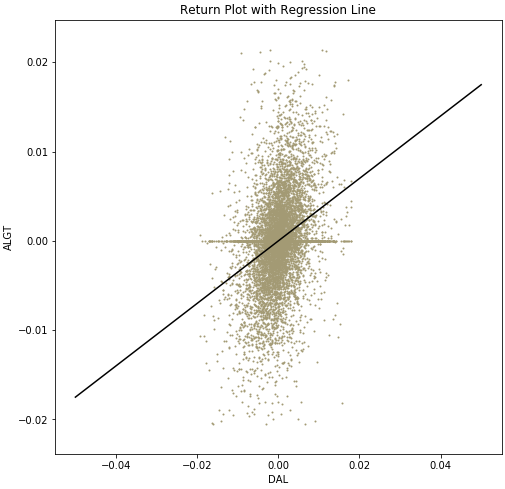
\includegraphics[width=.95\linewidth]{../Figures/return_plot_wReg.png}
    \caption{OLS Fit on No Outlier Data}
  \end{subfigure}%
  \begin{subfigure}{.5\textwidth}
    \centering
    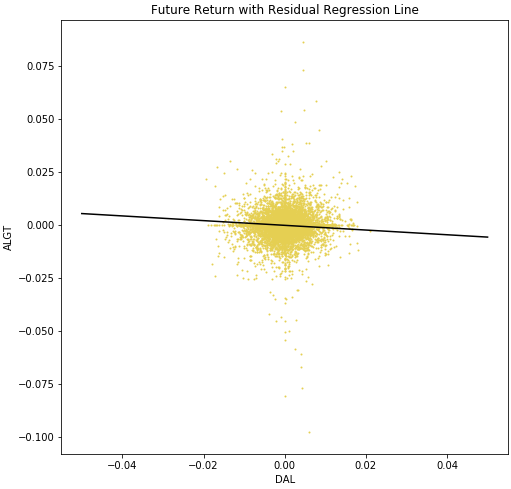
\includegraphics[width=.95\linewidth]{../Figures/return_plot_wResidReg.png}
    \caption{Future Returns Regressed on Model residuals}
  \end{subfigure}
  \caption{Return Plots with Regression}
\end{figure}
Include regression plot, coefficient plots
\subsection{Profit and Loss Analysis}
Introduce cumulative markout sums and parameter tuning.
include the PNl curves, and some pnl heatmaps
comment on allegiant

\section{Principal Component Basket Mean Reversion}
overview of goal and intuition here
\subsection{Dimensionality Reduction}
variance explained - show plots of first 4 PCs
correlation with returns
anomalies with coefficients
\subsection{Basket OLS}
Describe fit and any coefficient plots here
describe feature selection
\subsection{Basket Lasso for Feature Selection}
Omit this - mention briefly
\subsection{Profit and Loss Analysis}
plots of some pnls, also buying and selling matrices
Discuss why there is shortfall

\section{Discussion}
discuss shortfall of full strategy and why this might have occurred
dangers of assuming things revert to mean, mention correlation breakdowns during
covid
mention statistical issues with fit - high Dimensionality and lasso doing 
a poor job of feature selection because there are so many data points close to the 
0,0

\section{Conclusion}
highlight what was accomplished and what takeaways and next steps are

\newpage
\section{Appendix}

\subsection{RMSE for PC Regression Models}
\begin{table}[!htb]
    \begin{minipage}{.5\linewidth}
      \caption{Airline PC Regression RMSE}
      \centering
      \begin{tabular}{ c|c|c|c }
        \textbf{Ticker} & \textbf{PC1} & \textbf{Full} & \textbf{Lasso} \\
        \hline
        AAL	& 0.003519 & 0.003487 & 0.003487\\
        DAL	& 0.002762 & 0.002725 & 0.002725\\
        LUV	& 0.002839 & 0.002819 & 0.002819\\
        ALGT & 0.003561 & 0.003554 & 0.003554\\
        UAL	& 0.002931 & 0.002902 & 0.002902\\
        \end{tabular}
    \end{minipage}%
    \begin{minipage}{.5\linewidth}
      \centering
        \caption{Oil PC Regression RMSE}
        \begin{tabular}{ c|c|c|c  }
            \textbf{Ticker} & \textbf{PC1} & \textbf{Full} & \textbf{Lasso} \\
            \hline
            CVX	& 0.002338	& 0.002136	& 0.002136\\
            MRO	& 0.004708	& 0.004647	& 0.004647\\
            MUR	& 0.004573	& 0.004536	& 0.004536\\
            XOM	& 0.002240	& 0.002047	& 0.002047\\
            DVN	& 0.004302	& 0.004281	& 0.004284\\
        \end{tabular}
    \end{minipage} 
\end{table}

\begin{table}[!htb]
    \begin{minipage}{.5\linewidth}
      \caption{Airline and Oil PC Regression RMSE}
      \centering
      \begin{tabular}{ c|c|c|c }
        \textbf{Ticker} & \textbf{PC1} & \textbf{Full} & \textbf{Lasso} \\
        \hline
        AAL	& 0.004306	& 0.003475	& 0.003478\\
        DAL	& 0.003450	& 0.002721	& 0.002722\\
        LUV	& 0.003363	& 0.002809	& 0.002809\\
        ALGT & 0.003865	& 0.003552	& 0.003553\\
        UAL	& 0.003602	& 0.002896	& 0.002896\\
        CVX	& 0.002320	& 0.002124	& 0.002125\\
        MRO	& 0.004851	& 0.004640	& 0.004641\\
        MUR	& 0.004661	& 0.004530	& 0.004530\\
        XOM	& 0.002231	& 0.002044	& 0.002044\\
        DVN	& 0.004414	& 0.004275	& 0.004278\\
        \end{tabular}
    \end{minipage}%
    \begin{minipage}{.5\linewidth}
      \centering
        \caption{Full PC Regression RMSE}
        \begin{tabular}{ c|c|c|c  }
            \textbf{Ticker} & \textbf{PC1} & \textbf{Full} & \textbf{Lasso} \\
            \hline
            AAL	& 0.004301	& 0.003458	& 0.003458\\
            DAL	& 0.003446	& 0.002713	& 0.002713\\
            LUV	& 0.003359	& 0.002801	& 0.002801\\
            ALGT & 0.003863	& 0.003543	& 0.003545\\
            UAL	& 0.003598	& 0.002891	& 0.002891\\
            CVX	& 0.002316	& 0.002104	& 0.002105\\
            MRO	& 0.004854	& 0.004634	& 0.004635\\
            MUR	& 0.004666	& 0.004530	& 0.004531\\
            XOM	& 0.002227	& 0.001996	& 0.001996\\
            DVN	& 0.004418	& 0.004271	& 0.004275\\
            SPY	& 0.001469	& 0.001329	& 0.001330\\
            TLT	& 0.001574	& 0.001546	& 0.001546\\
        \end{tabular}
    \end{minipage} 
\end{table}

\newpage
\subsection{Return Plots}
\begin{figure}[h!]
  \centering
  \begin{subfigure}{.5\textwidth}
    \centering
    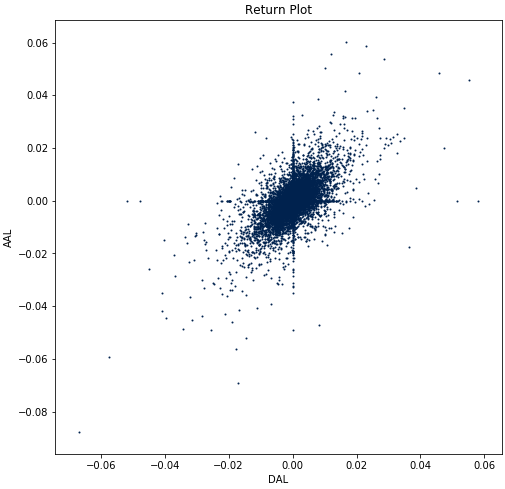
\includegraphics[width=.95\linewidth]{../Figures/return_plot_out.png}
    \caption{Returns with Outliers}
  \end{subfigure}%
  \begin{subfigure}{.5\textwidth}
    \centering
    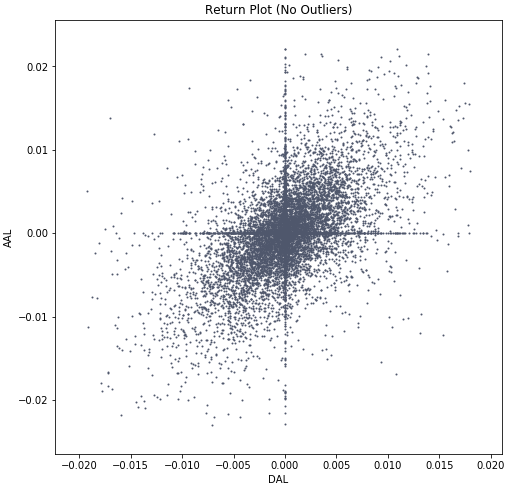
\includegraphics[width=.95\linewidth]{../Figures/return_plot_no_out.png}
    \caption{Returns with Outliers Removed}
  \end{subfigure}
  \caption{Impact of Outliers on Data}
\end{figure}

\begin{figure}[h!]
  \centering
  \begin{subfigure}{.5\textwidth}
    \centering
    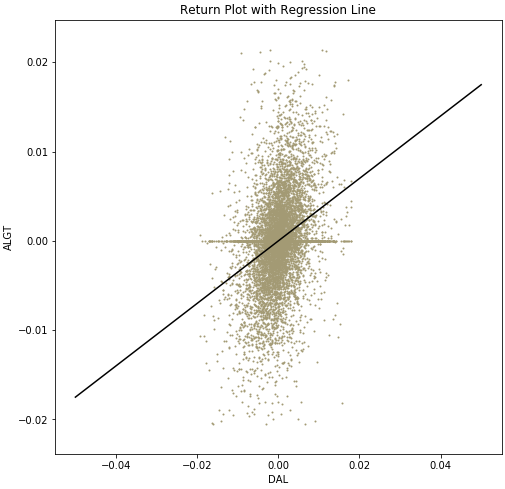
\includegraphics[width=.95\linewidth]{../Figures/return_plot_wReg.png}
    \caption{OLS Fit on No Outlier Data}
  \end{subfigure}%
  \begin{subfigure}{.5\textwidth}
    \centering
    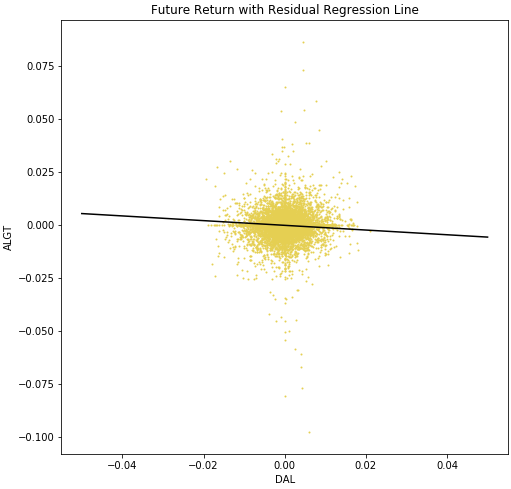
\includegraphics[width=.95\linewidth]{../Figures/return_plot_wResidReg.png}
    \caption{Future Returns Regressed on Model residuals}
  \end{subfigure}
  \caption{Return Plots with Regression}
\end{figure}

\newpage
\subsection{Correlations}
\begin{figure}[h!]
  \centering
    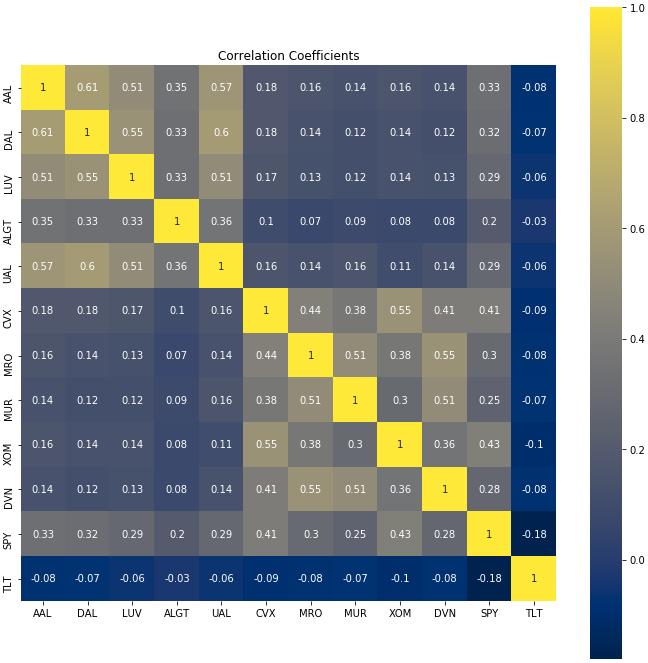
\includegraphics[width=.5\linewidth]{../Figures/pair_corr_out.png}
    \caption{Pairwise Correlation - Outliers Present}
\end{figure}
\begin{figure}[h!]
  \centering
    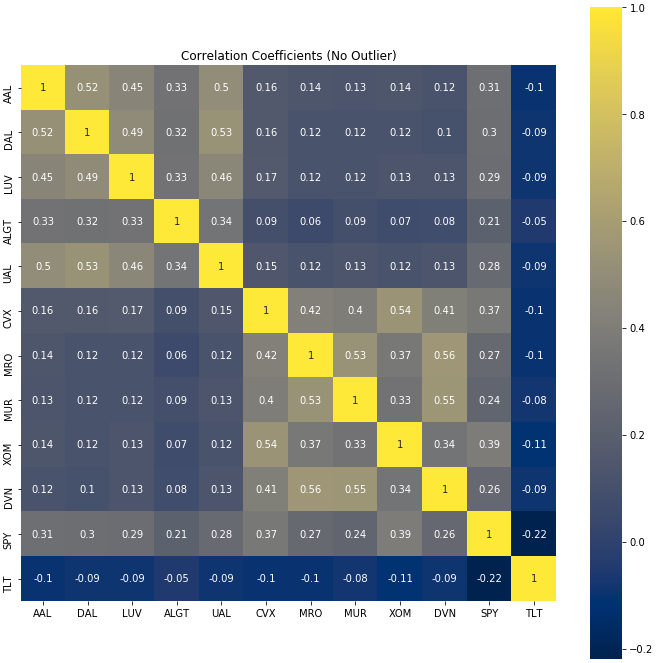
\includegraphics[width=.5\linewidth]{../Figures/pair_corr_no_out.png}
    \caption{Pairwise Correlation - Outliers Removed}
\end{figure}

\newpage
\subsection{Principal Component Analysis}
\begin{figure}[h!]
  \centering
    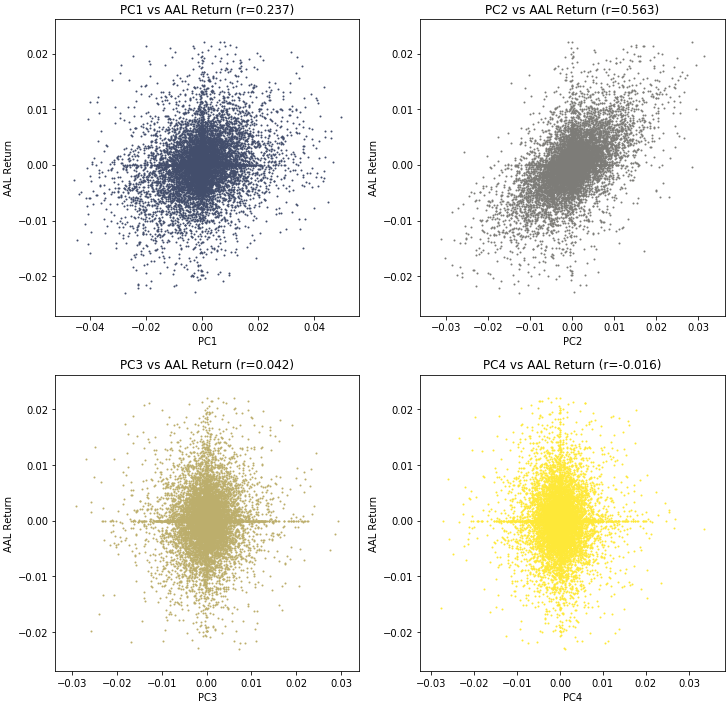
\includegraphics[width=.8\linewidth]{../Figures/PCA_plot.png}
    \caption{Decomposition Plot}
\end{figure}
\begin{figure}[h!]
  \centering
  \begin{subfigure}{.5\textwidth}
    \centering
    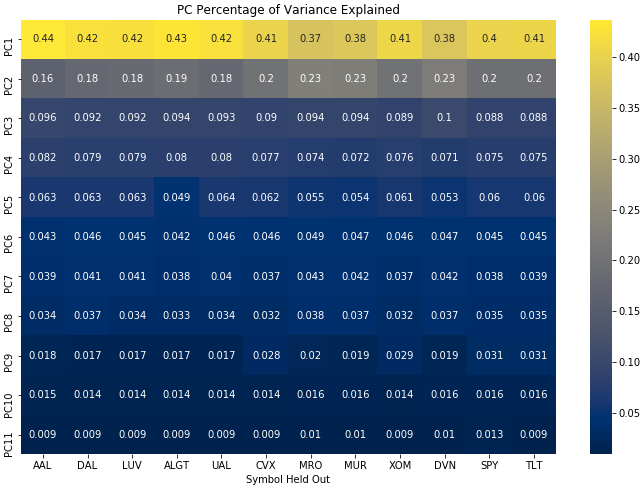
\includegraphics[width=.95\linewidth]{../Figures/PCA_pve.png}
    \caption{PCA Percentage of Variance Explained}
  \end{subfigure}%
  \begin{subfigure}{.5\textwidth}
    \centering
    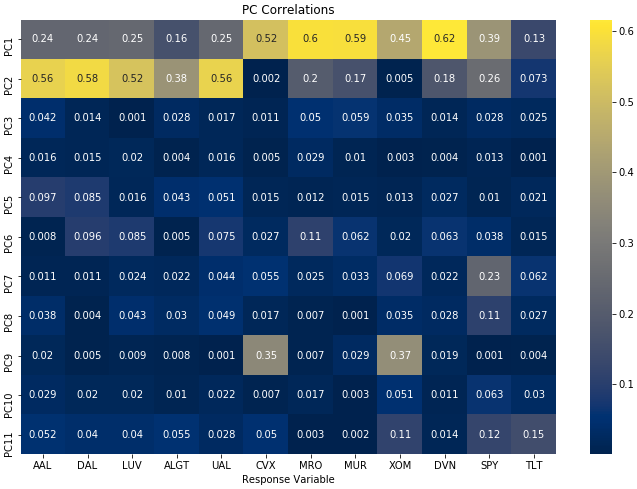
\includegraphics[width=.95\linewidth]{../Figures/PCA_corr_resp.png}
    \caption{Principal Component Correlation with Response}
  \end{subfigure}
  \caption{PCA Metrics}
\end{figure}

\newpage
\subsection{Regression Coefficients}

\subsubsection{Pairwise Regression}
\begin{figure}[h!]
  \centering
  \begin{subfigure}{.5\textwidth}
    \centering
    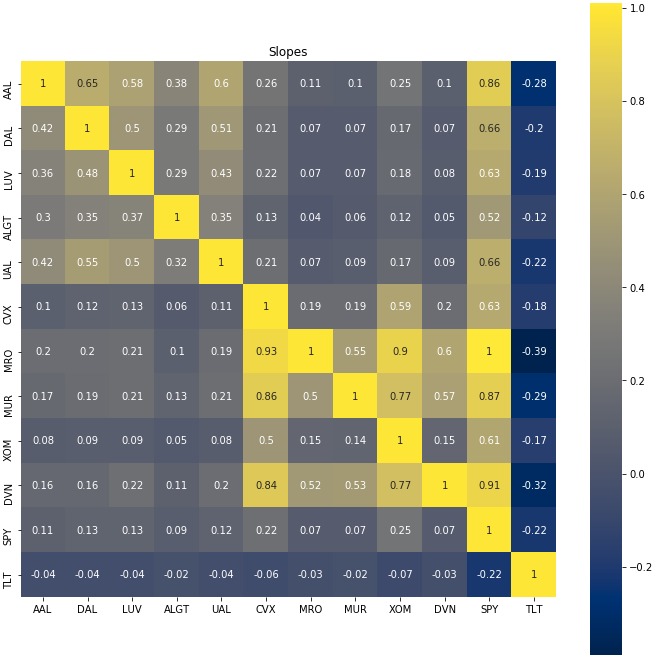
\includegraphics[width=.95\linewidth]{../Figures/pair_reg_slope.png}
    \caption{Slope Coefficient}
  \end{subfigure}%
  \begin{subfigure}{.5\textwidth}
    \centering
    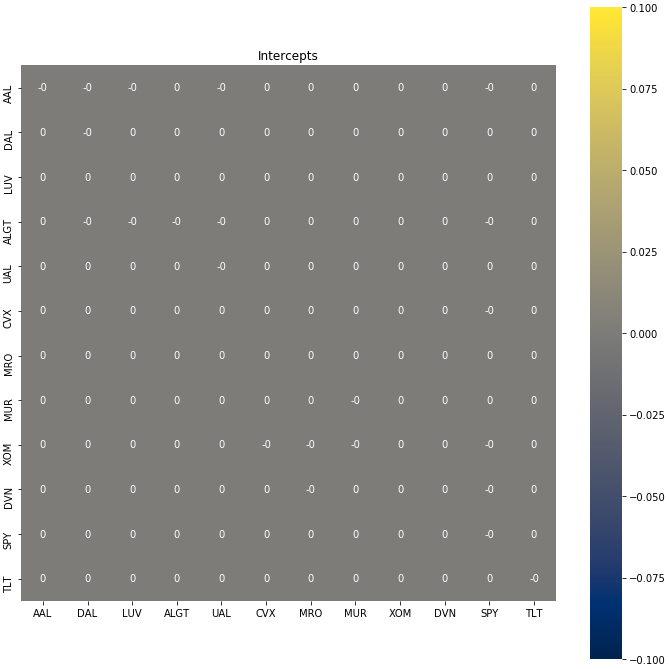
\includegraphics[width=.95\linewidth]{../Figures/pair_reg_intercept.png}
    \caption{Intercept}
  \end{subfigure}
  \caption{Pairwise Regression}
\end{figure}

\subsubsection{Pairwise Residual Regression}
\begin{figure}[h!]
  \centering
  \begin{subfigure}{.5\textwidth}
    \centering
    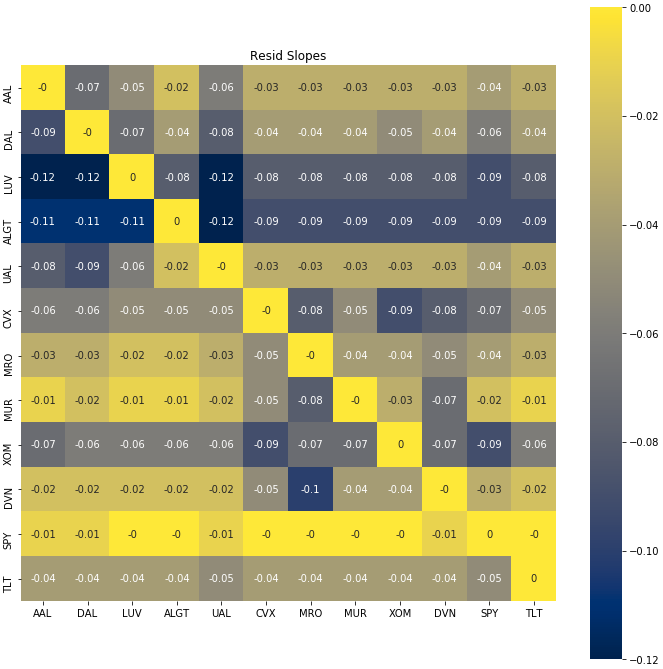
\includegraphics[width=.95\linewidth]{../Figures/pair_resid_reg_slope.png}
    \caption{Slope Coefficient}
  \end{subfigure}%
  \begin{subfigure}{.5\textwidth}
    \centering
    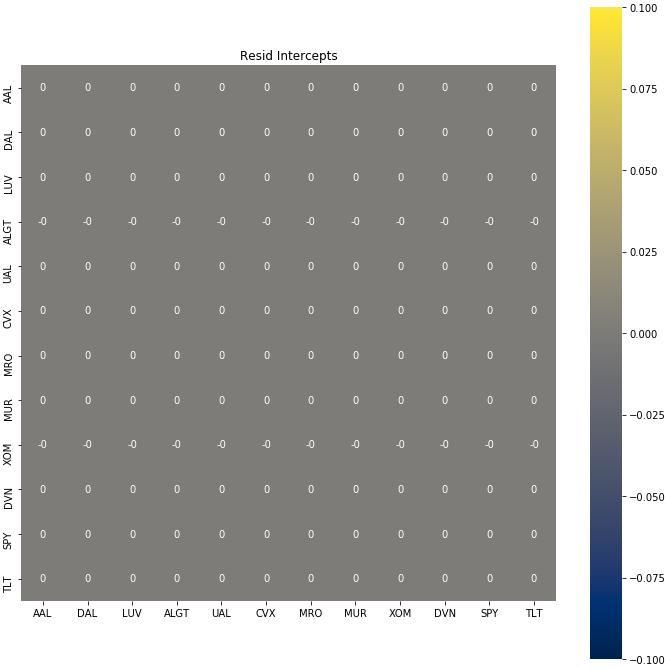
\includegraphics[width=.95\linewidth]{../Figures/pair_resid_reg_intercept.png}
    \caption{Intercept}
  \end{subfigure}
  \caption{Pairwise Residual Regression}
\end{figure}

\subsubsection{Principal Component Regression}
\begin{figure}[h!]
  \centering
    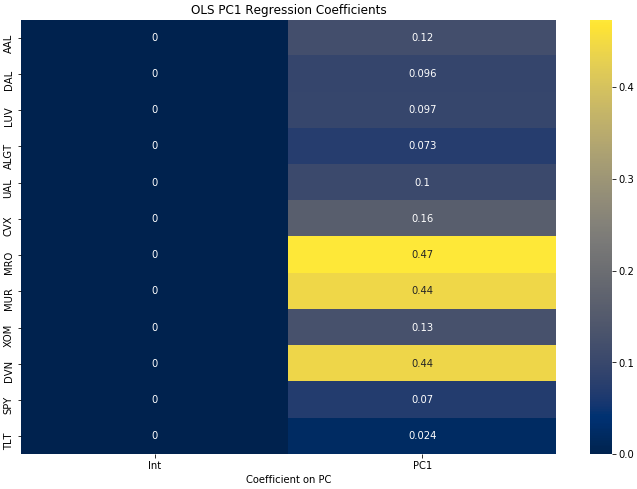
\includegraphics[width=.4\linewidth]{../Figures/PC1_PCReg_coef.png}
    \caption{PC1 OLS Regression}
\end{figure}
\begin{figure}[h!]
    \centering
    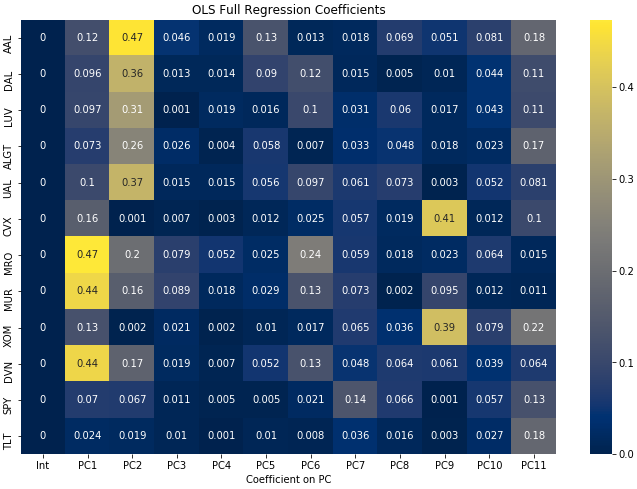
\includegraphics[width=.4\linewidth]{../Figures/Full_PCReg_coef.png}
    \caption{Full PC OLS Regression}
\end{figure}
\begin{figure}[h!]
    \centering
    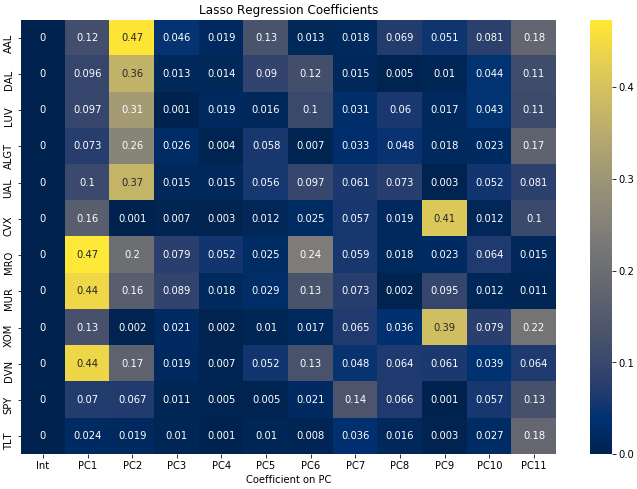
\includegraphics[width=.4\linewidth]{../Figures/Lasso_PCReg_coef.png}
    \caption{Lasso PC Regression}
\end{figure}

\newpage
\subsection{Profit and Loss Signal Curves}
\begin{figure}[h!]
  \centering
  \begin{subfigure}{.5\textwidth}
    \centering
    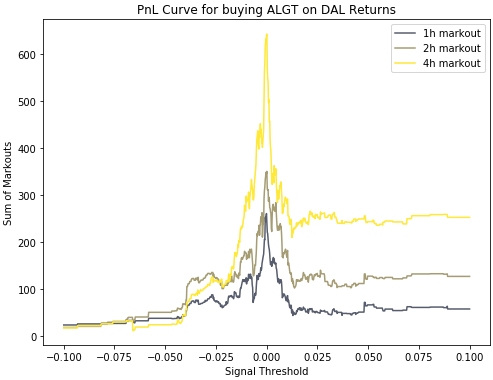
\includegraphics[width=.95\linewidth]{../Figures/pair_Pnl_Curve_buy_ALGT_on_DAL.png}
    \caption{Buy Side PnL}
  \end{subfigure}%
  \begin{subfigure}{.5\textwidth}
    \centering
    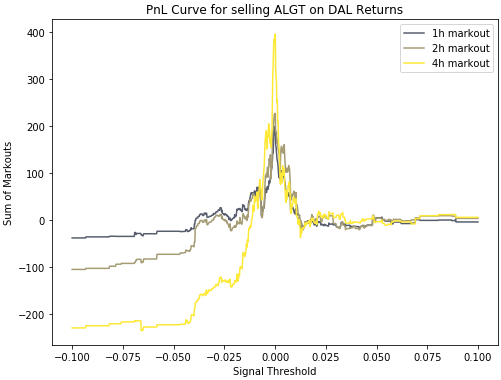
\includegraphics[width=.95\linewidth]{../Figures/pair_Pnl_Curve_sell_ALGT_on_DAL.png}
    \caption{Sell Side PnL}
  \end{subfigure}
  \caption{Pairwise Pnl Curves - ALGT}
\end{figure}

\begin{figure}[h!]
  \centering
  \begin{subfigure}{.5\textwidth}
    \centering
    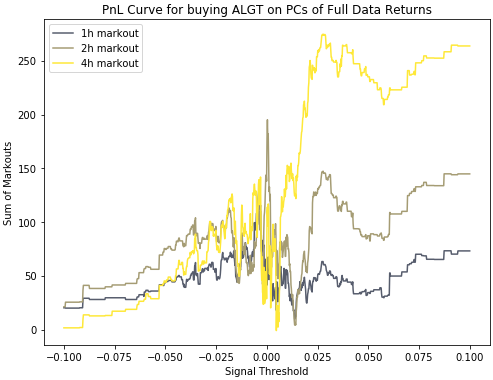
\includegraphics[width=.95\linewidth]{../Figures/basket_Pnl_Curve_buy_ALGT.png}
    \caption{Buy Side PnL}
  \end{subfigure}%
  \begin{subfigure}{.5\textwidth}
    \centering
    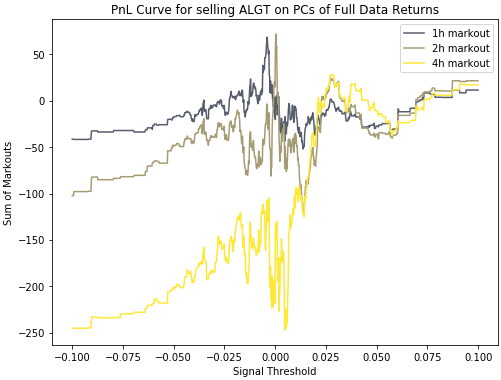
\includegraphics[width=.95\linewidth]{../Figures/basket_Pnl_Curve_sell_ALGT.png}
    \caption{Sell Side PnL}
  \end{subfigure}
  \caption{Basket Pnl Curves - ALGT}
\end{figure}

\newpage
\subsection{Profit and Loss over Markout Horizons}
\begin{figure}[h!]
  \centering
  \begin{subfigure}{.5\textwidth}
    \centering
    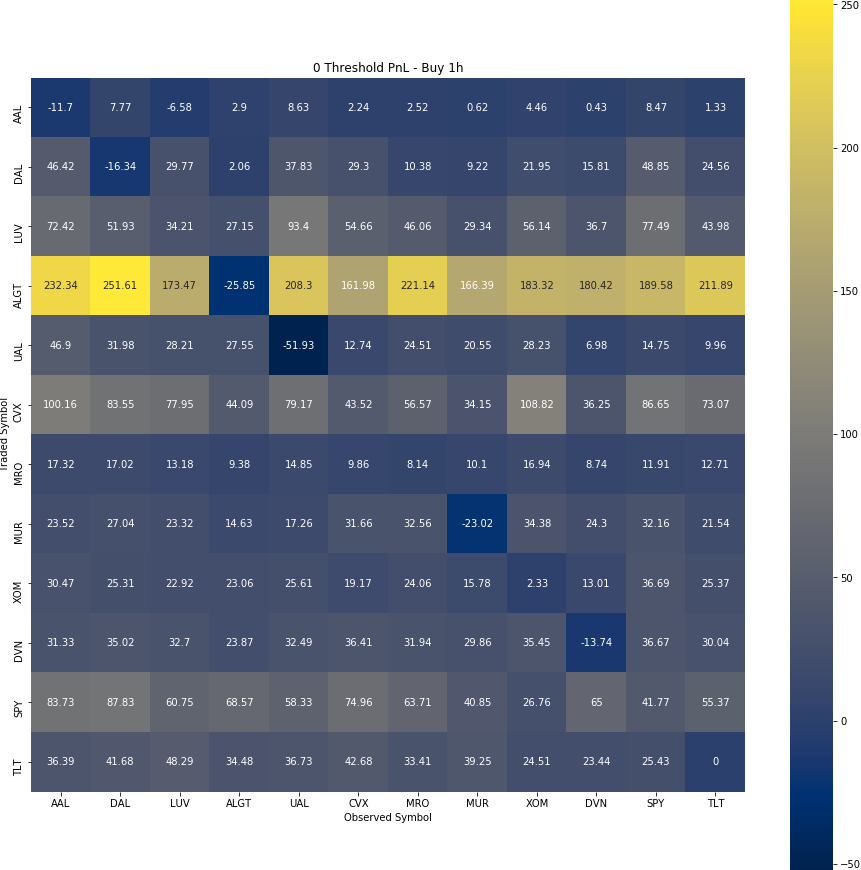
\includegraphics[width=.95\linewidth]{../Figures/pair_buy_pnl_1h.png}
    \caption{Buy Side PnL}
  \end{subfigure}%
  \begin{subfigure}{.5\textwidth}
    \centering
    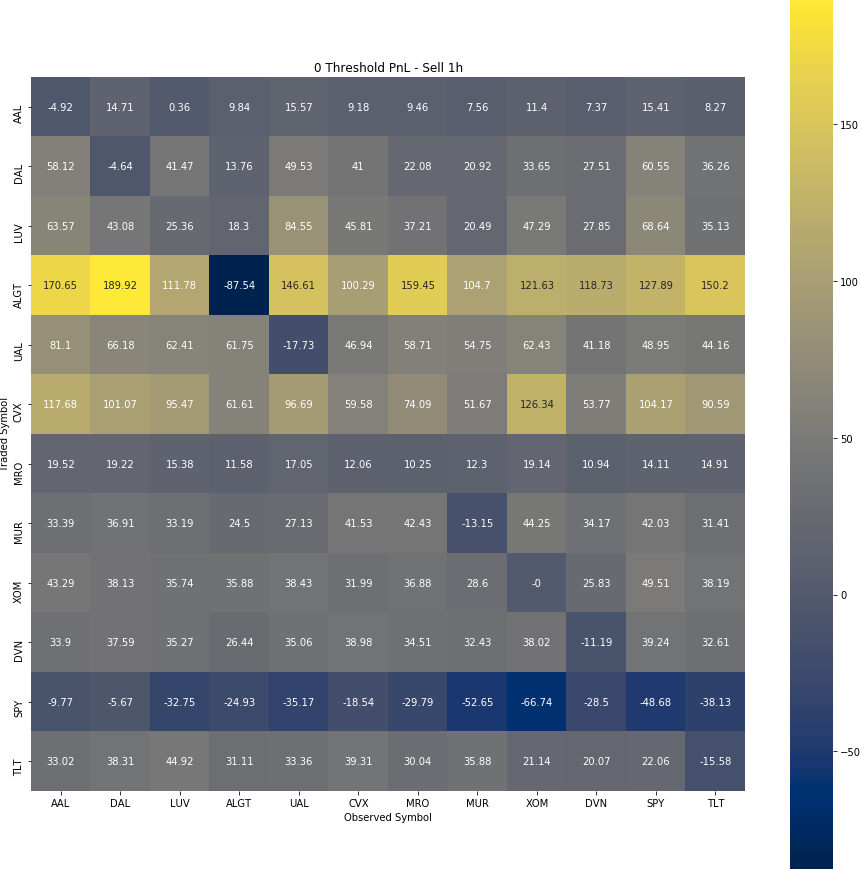
\includegraphics[width=.95\linewidth]{../Figures/pair_sell_pnl_1h.png}
    \caption{Sell Side PnL}
  \end{subfigure}
  \caption{1-Hour Markouts}
\end{figure}

\begin{figure}[h!]
  \centering
  \begin{subfigure}{.5\textwidth}
    \centering
    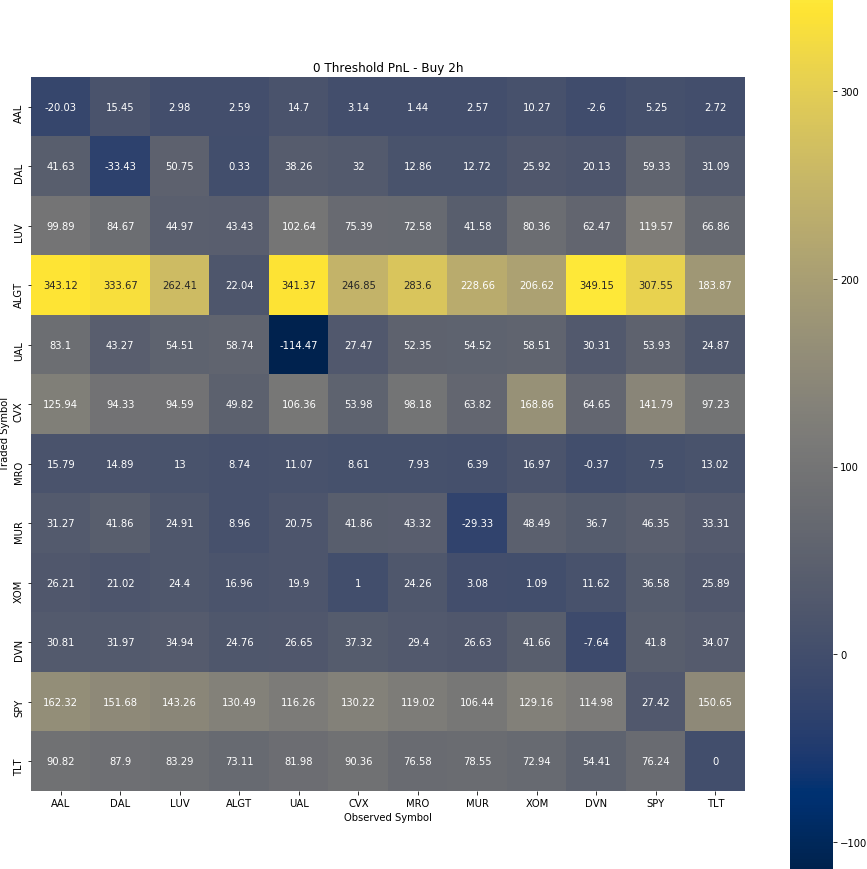
\includegraphics[width=.95\linewidth]{../Figures/pair_buy_pnl_2h.png}
    \caption{Buy Side PnL}
  \end{subfigure}%
  \begin{subfigure}{.5\textwidth}
    \centering
    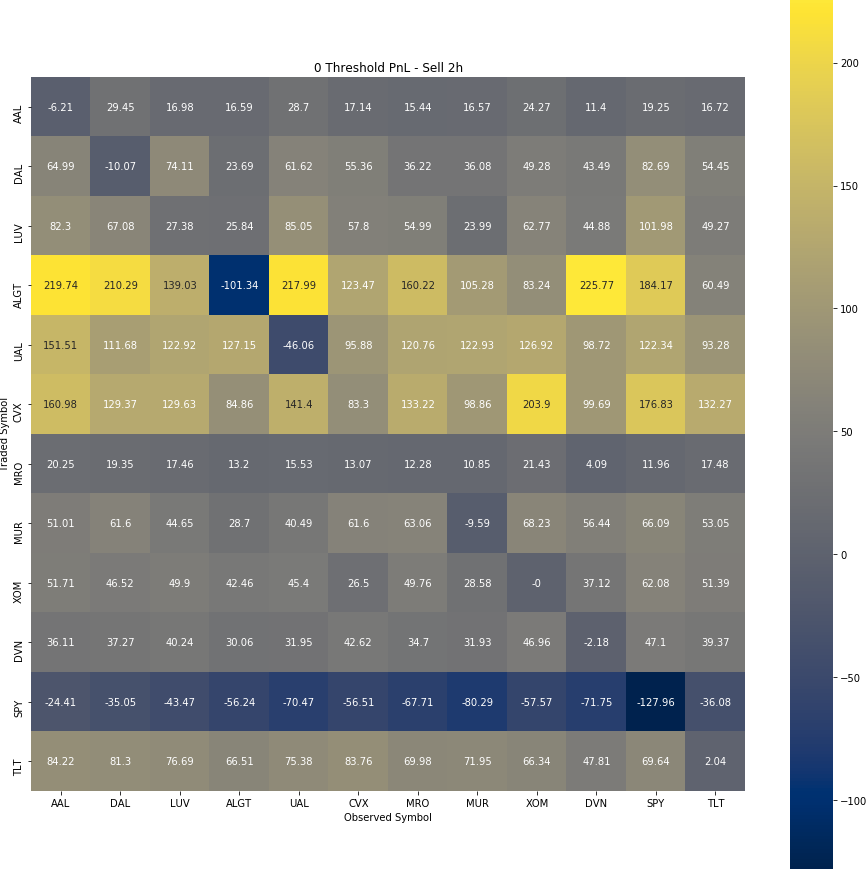
\includegraphics[width=.95\linewidth]{../Figures/pair_sell_pnl_2h.png}
    \caption{Sell Side PnL}
  \end{subfigure}
  \caption{2-Hour Markouts}
\end{figure}

\begin{figure}[h!]
  \centering
  \begin{subfigure}{.5\textwidth}
    \centering
    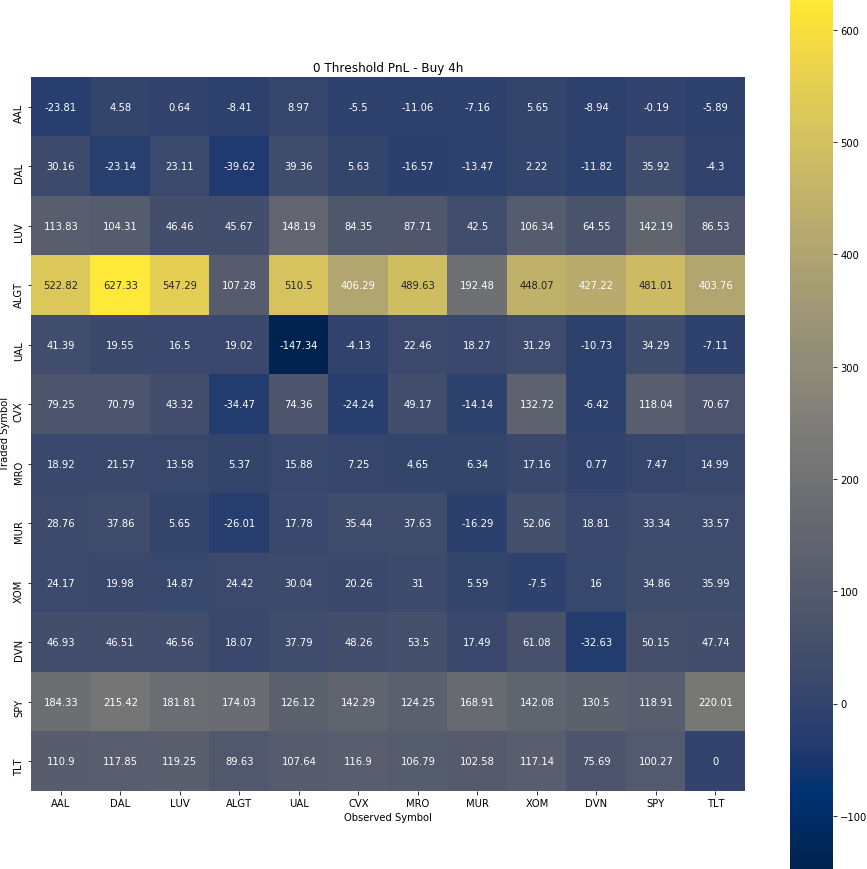
\includegraphics[width=.95\linewidth]{../Figures/pair_buy_pnl_4h.png}
    \caption{Buy Side PnL}
  \end{subfigure}%
  \begin{subfigure}{.5\textwidth}
    \centering
    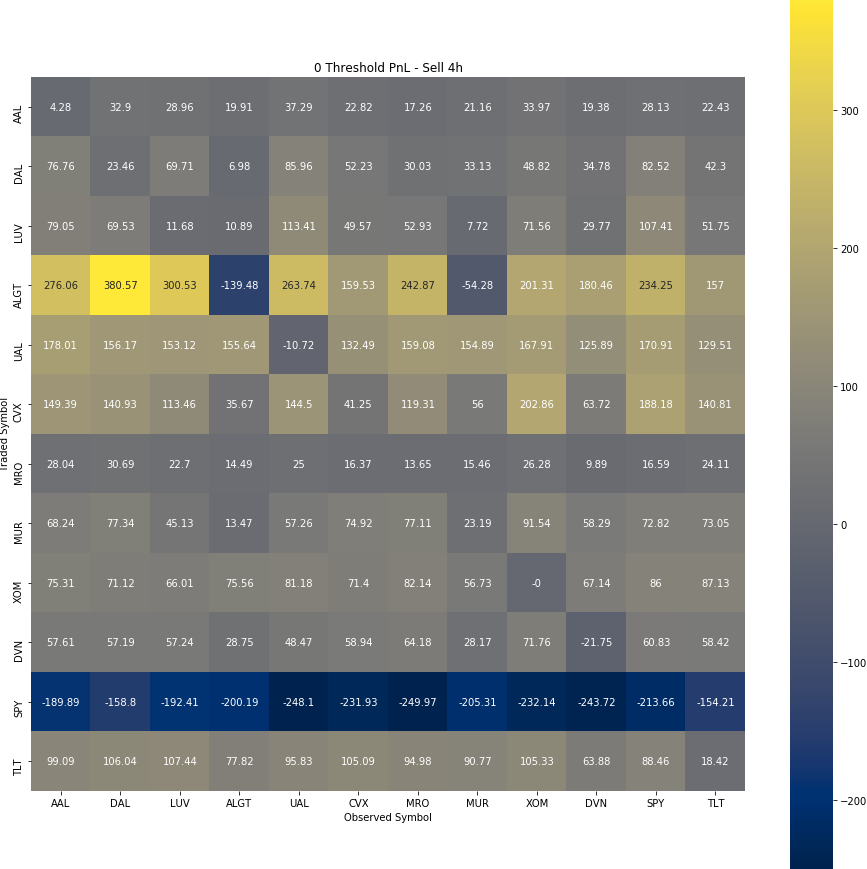
\includegraphics[width=.95\linewidth]{../Figures/pair_sell_pnl_4h.png}
    \caption{Sell Side PnL}
  \end{subfigure}
  \caption{4-Hour Markouts}
\end{figure}

\begin{figure}[h!]
  \centering
  \begin{subfigure}{.5\textwidth}
    \centering
    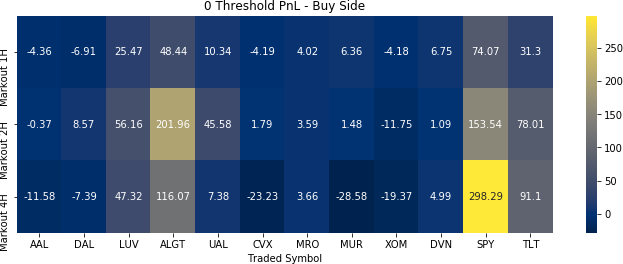
\includegraphics[width=.95\linewidth]{../Figures/basket_buy_pnl.png}
    \caption{Buy Side PnL}
  \end{subfigure}%
  \begin{subfigure}{.5\textwidth}
    \centering
    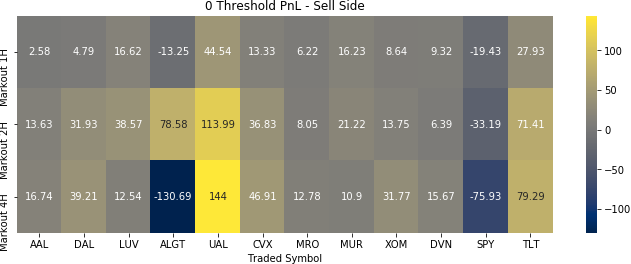
\includegraphics[width=.95\linewidth]{../Figures/basket_sell_pnl.png}
    \caption{Sell Side PnL}
  \end{subfigure}
  \caption{Basket Model PnL}
\end{figure}

\end{document}